\documentclass{article}
\title{Assignment \bf{ YoungDucks }}
\date{31.07.2013}
\usepackage[english]{babel}
\usepackage[cp1250]{inputenc}
\usepackage{hyperref}
\usepackage{enumerate}
\usepackage[cm,empty]{fullpage}
\usepackage[pdftex]{graphicx,color}
\usepackage{Sweave}
\begin{document}
\maketitle{}
\section{ Data about the group }{\bf : }April Duck, May Duck, June Duck, Huey Duck, Dewey Duck, Louie Duck\\{\bf Due date : 15th of October 2012 }\\{\bf Sources : }Lecture Notes\\{\bf Template to use : Probability.doc }\\\section{ Assignment }
A genetically modified mouse does not survive the first month of life with probability 0.3 . \\\begin{itemize}
\item  We planned an experiment that included 7 mice. What is the probability that after a month not more than a mouse will survive? 
\item What is the expected number of mice still alive after the first month? 
\item Is the animal represented in the picture a genetically modified mouse?
\begin{tabular}{c}
\resizebox{50mm}{!}{
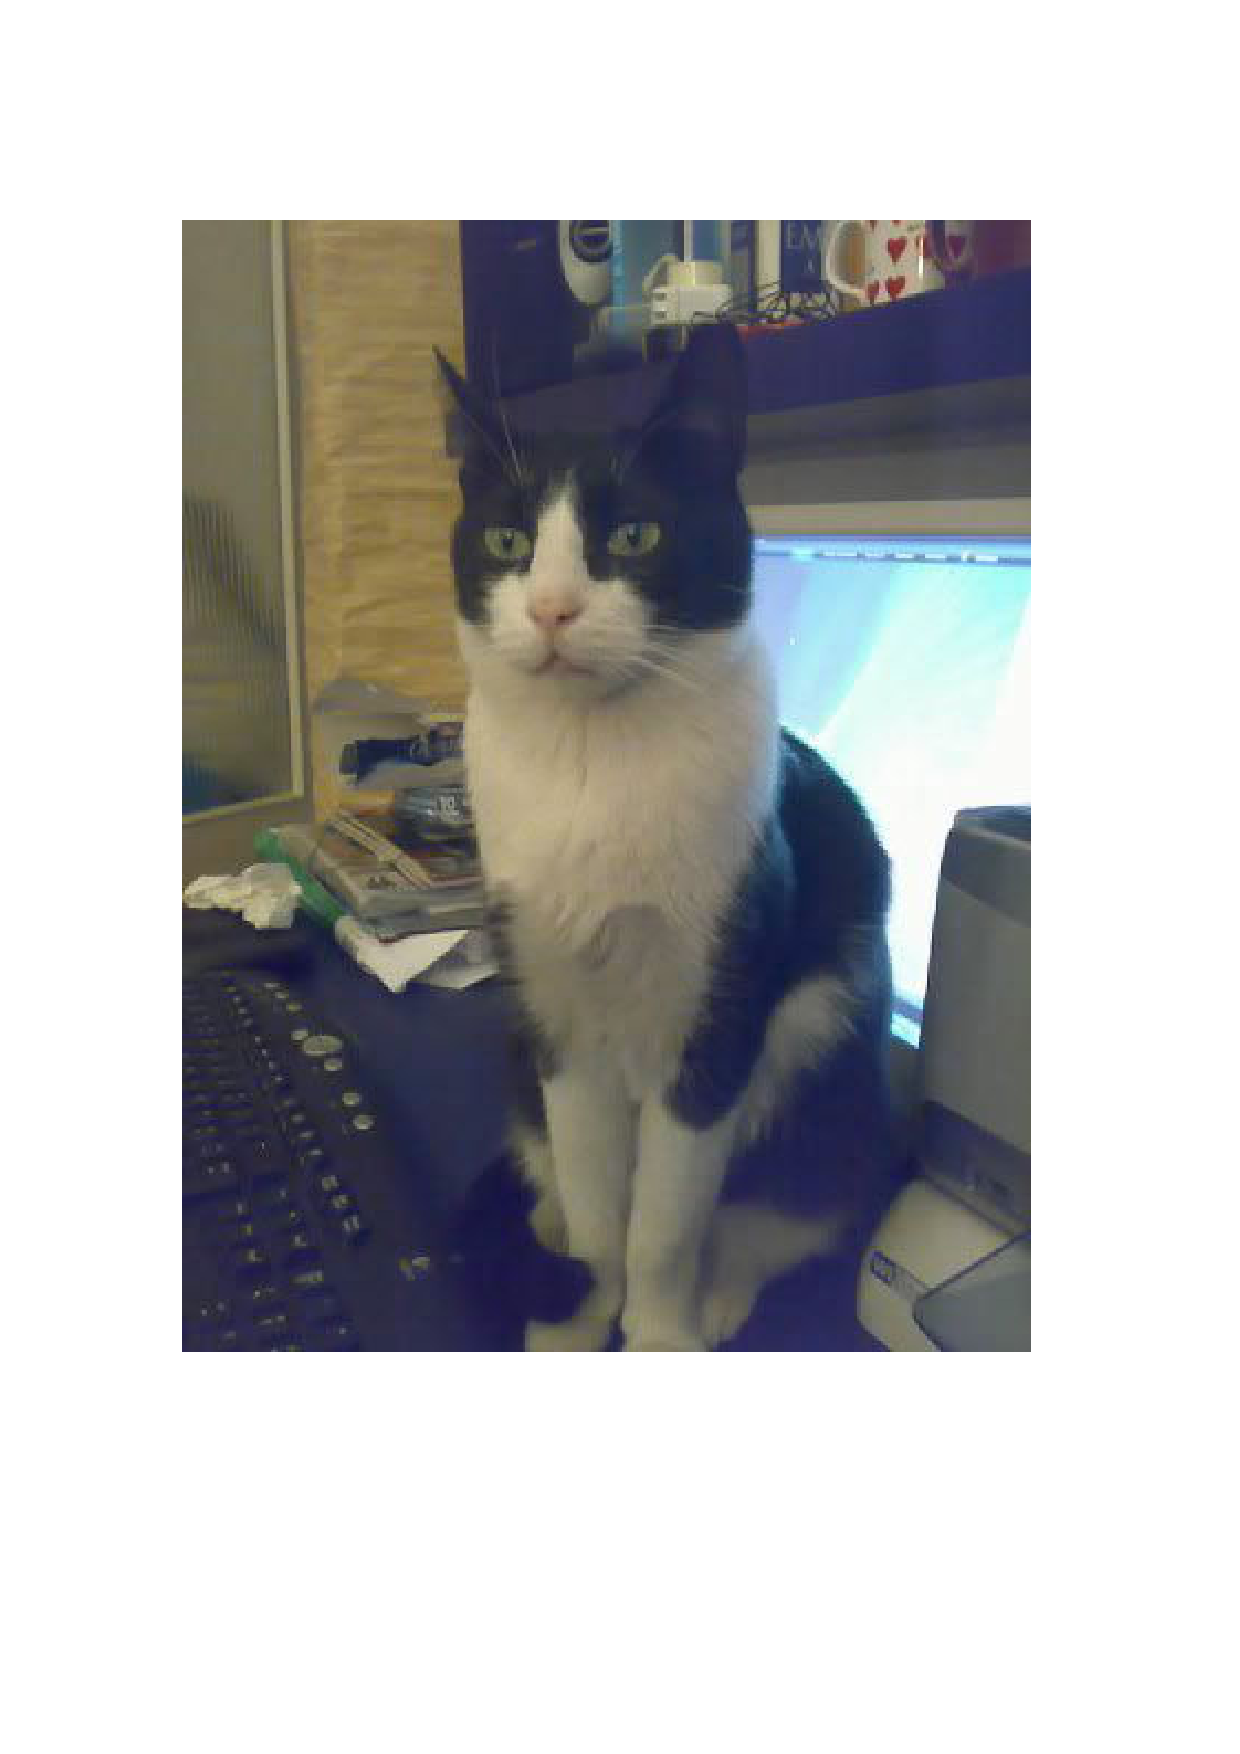
\includegraphics{yoyopdf}
}
\end{tabular} 
\end{itemize}
\vspace{\baselineskip} {\bf Good luck! }\newpage
\end{document}
